\chapter{أنتالبيات التفاعل}\label{ch:b2:reaction-enthalpy}

خرطوشة غاز تخييم مثبّتة تحت موقد صغير: بضعة غرامات من البوتان تُغلي
لترًا من الماء في دقائق، واللهب الأزرق تحت القدر أسخن بكثير من الماء
المغلي. ما مقدار الحرارة التي يحررها التفاعل، وكم منها يصل إلى القدر،
وإلى أي حدّ يمكن أن ترتفع درجة حرارة اللهب؟ لا يحتاج أي من هذه الأسئلة
إلى موقد للإجابة عنه: فجداول تضم بضعة أعداد لكل مادة، تُقاس مرة واحدة
وإلى الأبد، تعطي حرارة كل تفاعل يمكن كتابته بهذه المواد، عند أي درجة
حرارة. يبني هذا الفصل هذه المحاسبة. فهو يطبّق المبدأ الأول في
الترموديناميك، المعروف من الفيزياء، على نظام يتغير تركيبه، ويعرّف \omterm{def:b2:reaction-enthalpy:reaction-quantity}{أنتالبي
التفاعل} مشتقةً جزئية، ويبيّن كيف يُحسب من أنتالبيات التكوين ومن
أنتالبيات الروابط وعبر الدورات، وكيف يتغير مع درجة الحرارة، وماذا يقول
عن اللهب وعن المساعر.

\begin{recall}
من الفيزياء: المبدأ الأول $\Delta U = W + Q$؛ والأنتالبي $H = U + pV$،
وهو دالة حالة؛ وعند ضغط خارجي ثابت، وبين حالتين عند هذا الضغط، تكون
الحرارة المستقبَلة $Q_p = \Delta H$؛ والسعة الحرارية عند ضغط ثابت
$C_p = (\partial H/\partial T)_p$؛ وأنتالبي الغاز المثالي لا يتعلق إلا
بدرجة الحرارة $T$. ووصف مجلد السنة الأولى نظامًا متفاعلًا بتقدمه $\xi$
وبالأعداد الستوكيومترية $\nu_i$ في المعادلة
$0 = \sum_i\nu_i\mathrm A_i$، وثبّت الحالة القياسية لكل نوع كيميائي
عند $p^\circ = \qty{1}{bar}$. وسمّى المجلد المدرسي (الصف 11) التفاعلَ
\omterm{def:b2:reaction-enthalpy:exothermic}{ناشرًا للحرارة} حين يحرر حرارة، وقدّر طاقات الاحتراق من طاقات
الروابط.
\end{recall}

\begin{omfigure}
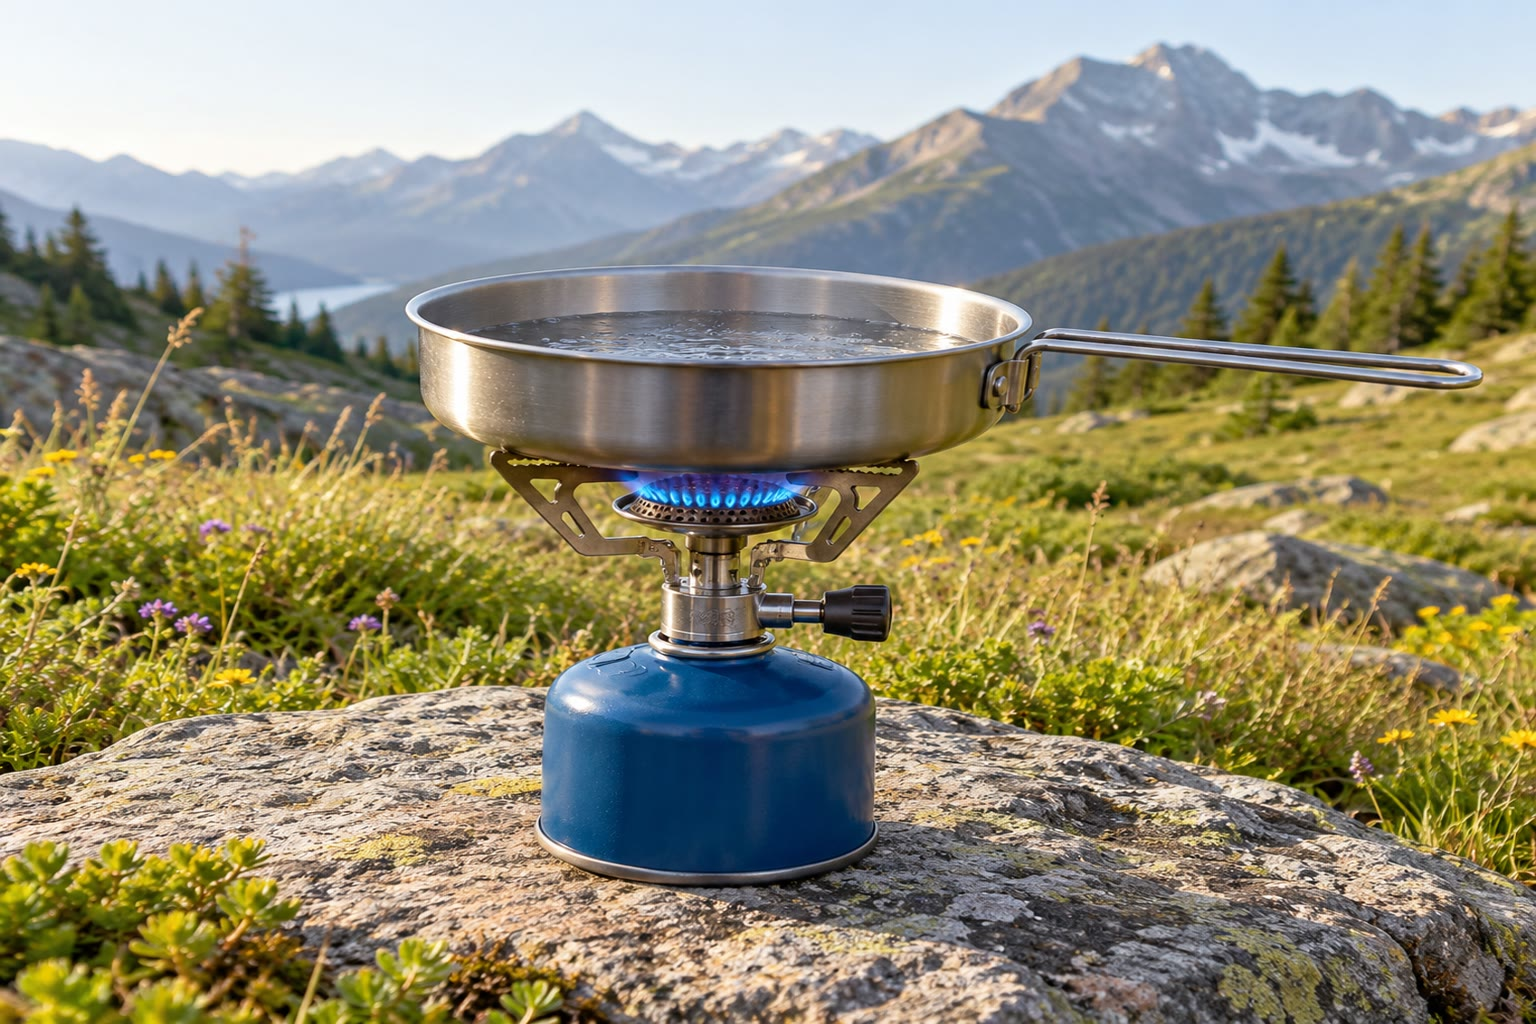
\includegraphics[width=0.6\linewidth]{images/book3/ai/b2-01-camping-stove.jpg}

{\small موقد تخييم: يحترق البوتان الآتي من الخرطوشة في الهواء تحت
القدر. وتُحسب في مسألة نهاية الأسبوع لهذا الفصل الحرارةُ المحررة لكل
مول من البوتان، والحصة التي تصل منها إلى الماء، ودرجة حرارة
اللهب.}
\end{omfigure}

\section{مقادير التفاعل}

يوصف نظام مغلق يجري فيه التفاعل الوحيد $0 = \sum_i\nu_i\mathrm A_i$
بدرجة حرارته وضغطه وتقدمه: فكميات المادة هي $n_i = n_{i,0} + \nu_i\xi$.
وكل دالة حالة ممتدة للنظام، أنتالبيه مثلًا، هي عندئذ دالة $H(T, p,
\xi)$، وتفاضلها التام هو
\[
  \dd H = \left(\frac{\partial H}{\partial T}\right)_{p,\xi}\dd T
        + \left(\frac{\partial H}{\partial p}\right)_{T,\xi}\dd p
        + \left(\frac{\partial H}{\partial \xi}\right)_{T,p}\dd\xi .
\]

\begin{definition}[مقدار التفاعل، أنتالبي التفاعل]\label{def:b2:reaction-enthalpy:reaction-quantity}
من أجل دالة حالة ممتدة $X$ لنظام مغلق يجري فيه التفاعل
$0 = \sum_i\nu_i\mathrm A_i$، يكون \emph{مقدار التفاعل}\index{مقدار التفاعل}
هو المشتقة الجزئية
\[
  \Delta_r X = \left(\frac{\partial X}{\partial \xi}\right)_{T,p} ,
\]
أي تغيّر $X$ لكل وحدة تقدم عند درجة حرارة وضغط ثابتين، بوحدة $X$ لكل
مول. ومن أجل $X = H$ هو \emph{أنتالبي التفاعل}\index{أنتالبي التفاعل}
$\Delta_r H$، بوحدة \unit{kJ/mol}.
\end{definition}

\begin{remark}[مشتقة لا فرق]\label{rem:b2:reaction-enthalpy:operator}
الرمز $\Delta_r$ مؤثر: يُطبَّق على حالة النظام ويتركها دون تغيير.
وكتابة التفاعل على نحو آخر (بمضاعفة معاملاته) تضاعف $\Delta_r H$، فلا
معنى لمقدار تفاعل دون معادلته. وحين تُستعمل الأنتالبيات المولية الجزئية
$\bar H_i = (\partial H/\partial n_i)_{T,p,n_j}$ للأنواع الكيميائية
(\cref{ch:b2:chemical-potential})، يكون $\Delta_r H = \sum_i\nu_i\bar H_i$،
بقاعدة السلسلة مطبَّقةً على $n_i = n_{i,0} + \nu_i\xi$.
\end{remark}

\begin{proposition}[الحرارة المستقبَلة عند درجة حرارة وضغط ثابتين]\label{prop:b2:reaction-enthalpy:qp}
حين يتقدم التفاعل من $\xi_1$ إلى $\xi_2$ في نظام محفوظ عند $T$ و$p$
ثابتين، يستقبل النظام الحرارة
\[
  Q_p = \int_{\xi_1}^{\xi_2}\Delta_r H\,\dd\xi = \Delta_r H\,(\xi_2 - \xi_1)
\]
إذا لم يتعلق $\Delta_r H$ بالتقدم $\xi$.
\end{proposition}

\begin{proof}
عند $p$ ثابت (وهنا عند ضغط خارجي ثابت أيضًا)، تكون الحرارة المستقبَلة
هي تغير الأنتالبي، $Q_p = \Delta H$ (الفيزياء). وعند $T$ و$p$ مثبّتين
يؤول تفاضل $H$ إلى $\dd H = \Delta_r H\,\dd\xi$؛ وبالمكاملة من $\xi_1$
إلى $\xi_2$ نحصل على النتيجة.
\end{proof}

\begin{definition}[ناشر للحرارة، ماص للحرارة، لاحراري]\label{def:b2:reaction-enthalpy:exothermic}
يكون التفاعل \emph{ناشرًا للحرارة}\index{ناشر للحرارة} في حالة معيّنة إذا
كان $\Delta_r H < 0$: فإذا جرى في الاتجاه المباشر عند $T$ و$p$ ثابتين
أعطى حرارة للوسط المحيط. ويكون \emph{ماصًا للحرارة}\index{ماص للحرارة}
إذا كان $\Delta_r H >
0$، و\emph{لاحراريًا}\index{لاحراري} إذا كان $\Delta_r H = 0$.
\end{definition}

لا تتعلق حرارة التفاعل في الغالب بالتركيب: فمن أجل الغازات المثالية
والأجسام الصلبة والسوائل النقية، لا يتعلق أنتالبي كل نوع كيميائي بما
يحيط به، ويتحدد $\Delta_r H$ بمجرد تحديد $T$.

\begin{proposition}[الأنظمة المثالية]\label{prop:b2:reaction-enthalpy:ideal}
في خليط من الغازات المثالية مع أطوار مكثفة نقية، لا يتعلق $\Delta_r H$
إلا بدرجة الحرارة، ويساوي \omterm{def:b2:reaction-enthalpy:standard-reaction-enthalpy}{أنتالبي التفاعل القياسي} $\Delta_r H^\circ(T)$
المعرَّف أدناه. ومن أجل المذابات في محلول مخفف تتحقق المساواة بتقريب
جيد.
\end{proposition}

\begin{proof}
في خليط من الغازات المثالية يسلك كل غاز كما لو كان وحده، بأنتالبي
$n_iH_{m,i}(T)$ لا يتعلق بالضغط $p$ (الفيزياء: أنتالبي الغاز المثالي لا
يتعلق إلا بدرجة الحرارة $T$). وللجسم الصلب أو السائل النقي $H = n_iH_{m,i}(T,
p)$، والمقدار $(\partial H_m/\partial p)_T = V_m(1 - \alpha T)$ لا يتجاوز بضع
وحدات \unit{J/(mol.bar)} في طور مكثف، وهو مهمل أمام أنتالبيات تفاعل من
رتبة عشرات \unit{kJ/mol}. إذن $H = \sum_in_iH_{m,i}(T)$، ومشتقته بالنسبة
إلى $\xi$ هي $\sum_i\nu_iH_{m,i}(T)$: لا تتعلق إلا بالمتغير
$T$، وقيمتها هي القيمة المحسوبة وكل نوع كيميائي في حالته القياسية.
\end{proof}

\section{أنتالبيات التفاعل القياسية وقانون هس}

\begin{definition}[مقدار التفاعل القياسي]\label{def:b2:reaction-enthalpy:standard-reaction-enthalpy}
\emph{مقدار التفاعل القياسي}\index{مقدار التفاعل القياسي}
$\Delta_r X^\circ(T) = \sum_i\nu_iX_{m,i}^\circ(T)$ هو \omterm{def:b2:reaction-enthalpy:reaction-quantity}{مقدار التفاعل} المحسوب
وكل نوع كيميائي في حالته القياسية عند درجة الحرارة $T$، حيث
$X_{m,i}^\circ$ هي القيم المولية القياسية. ومن أجل $X = H$ هو
\emph{أنتالبي التفاعل القياسي}\index{أنتالبي التفاعل القياسي}
$\Delta_r H^\circ(T)$؛ ولا يتعلق إلا بدرجة الحرارة $T$.
\end{definition}

لا تُقاس إلا فروق الأنتالبي، فيُختار مرجع مرة واحدة وإلى الأبد، كما
اختير قطب الهيدروجين مرجعًا للجهود.

\begin{definition}[الحالة المرجعية القياسية، أنتالبي التكوين القياسي]\label{def:b2:reaction-enthalpy:formation}
\emph{الحالة المرجعية القياسية}\index{حالة مرجعية قياسية} لعنصر عند درجة
الحرارة $T$ هي أكثر أشكاله استقرارًا عند $T$ تحت الضغط $p^\circ$:
\ce{H2} و\ce{O2} و\ce{N2} و\ce{Cl2} غازاتٍ مثالية، والكربون غرافيتًا،
والصوديوم فلزًا، والبروم سائلًا (عند \qty{298}{K}).
و\emph{أنتالبي التكوين القياسي}\index{أنتالبي التكوين القياسي}
$\Delta_f H^\circ$ لمركب هو \omterm{def:b2:reaction-enthalpy:standard-reaction-enthalpy}{أنتالبي التفاعل القياسي} لتفاعل تكوينه، أي
التفاعل الذي يصنع مولًا واحدًا من المركب انطلاقًا من عناصره في حالاتها
المرجعية. وبحكم البناء، $\Delta_f H^\circ = 0$ لعنصر في حالته المرجعية.
\end{definition}

\begin{example}[تفاعلات التكوين]\label{ex:b2:reaction-enthalpy:formation}
تفاعل تكوين الماء هو \ce{H2(g) + 1/2O2(g) -> H2O(l)}، مع
$\Delta_f H^\circ = \qty{-285.83}{kJ/mol}$ عند \qty{298.15}{K}؛ وتفاعل تكوين
الميثان هو \ce{C(s) + 2H2(g) -> CH4(g)}، $\Delta_f H^\circ =
\qty{-74.9}{kJ/mol}$؛ وتفاعل تكوين أحادي أكسيد النيتروجين، \ce{1/2N2(g) + 1/2O2(g) ->
NO(g)}، $\Delta_f H^\circ = \qty{+90.3}{kJ/mol}$: مركب \omterm{def:b2:reaction-enthalpy:exothermic}{ماص للحرارة}،
تصنعه مع ذلك الغازات الساخنة في المحرك. ولا تطرح المعاملات النصفية أي
مشكلة: فتفاعل التكوين أداة محاسبية، لا آلية.
% ledger: dfh:H2O-l, dfh:CH4_g, dfh:NO_g
\end{example}

\begin{theorem}[قانون هس]\label{thm:b2:reaction-enthalpy:hess}
إذا كان تفاعل ما هو المجموع، بالمعاملات $\lambda_k$، للتفاعلات $k$، فإن
أنتالبي تفاعله القياسي هو التركيب نفسه لأنتالبياتها:
$\Delta_r H^\circ = \sum_k\lambda_k\Delta_r H_k^\circ$
(\emph{قانون هس}\index{قانون هس}). وبخاصة، يمكن حساب أنتالبي تفاعل قياسي
عبر أي مسار من التفاعلات يقود من المتفاعلات إلى النواتج.
\end{theorem}

\begin{proof}
كل $\Delta_r H_k^\circ = \sum_i\nu_{i,k}H_{m,i}^\circ$ خطي في الأعداد
الستوكيومترية. فإذا كان التفاعل هو التركيب $\sum_k\lambda_k$ للتفاعلات
$k$، كانت أعداده الستوكيومترية $\nu_i = \sum_k\lambda_k
\nu_{i,k}$، و$\Delta_r H^\circ = \sum_i\nu_iH_{m,i}^\circ = \sum_k\lambda_k
\sum_i\nu_{i,k}H_{m,i}^\circ$. ووراء هذا الجبر يقف المبدأ الأول: $H$ دالة
حالة، فتغيّرها بين الحالتين الابتدائية والنهائية نفسيهما لا يتعلق
بالمسار.
\end{proof}

\begin{proposition}[أنتالبي التفاعل من أنتالبيات التكوين]\label{prop:b2:reaction-enthalpy:formation-sum}
$\Delta_r H^\circ(T) = \sum_i\nu_i\,\Delta_f H_i^\circ(T)$.
\end{proposition}

\begin{proof}
لنأخذ المسار الذي يفكك المتفاعلات إلى عناصرها في حالاتها المرجعية (عكس
تفاعلات تكوينها، بالمعاملات $-\nu_i > 0$)، ثم يكوّن النواتج من العناصر
نفسها (بالمعاملات $\nu_i > 0$). تُختصر العناصر لأن المعادلة موزونة،
ويجمع \omterm{thm:b2:reaction-enthalpy:hess}{قانون هس} الأنتالبيات.
\end{proof}

\begin{omfigure}
\begin{tikzpicture}[font=\small, >={Stealth}, y=0.0062cm]
  \draw[->] (0,-1000) -- (0,180) node[above] {\babelsublr{$H^\circ$ (\unit{kJ/mol})}};
  \foreach \y in {0,-200,-400,-600,-800,-1000} \draw (-0.08,\y) -- (0.08,\y) node[left=4pt] {$\y$};
  % levels
  \draw[very thick] (1.0,0) -- (4.6,0) node[right] {\ce{C(s) + 2H2(g) + 2O2(g)}};
  \draw[very thick, omDef] (1.0,-74.9) -- (4.6,-74.9);
  \node[right, omDef] at (4.6,-110) {\ce{CH4(g) + 2O2(g)}};
  \draw[very thick, omThm] (1.0,-965.2) -- (4.6,-965.2) node[right] {\ce{CO2(g) + 2H2O(l)}};
  % arrows
  \draw[->, omDef, thick] (1.6,0) -- (1.6,-74.9);
  \node[omDef, anchor=south west, font=\footnotesize] at (1.1,5) {$\Delta_f H^\circ(\ce{CH4}) = -74.9$};
  \draw[->, omThm, thick] (3.9,0) -- (3.9,-965.2);
  \node[right, omThm, align=left] at (3.95,-500) {$\Delta_f H^\circ(\ce{CO2})$\\ $+ 2\Delta_f H^\circ(\ce{H2O})$\\ $= -965.2$};
  \draw[->, thick] (2.75,-74.9) -- (2.75,-965.2);
  \node[left, align=right] at (2.7,-650) {$\Delta_r H^\circ$\\ $= -890.3$};
\end{tikzpicture}

{\small مستويات الأنتالبي لاحتراق الميثان عند \qty{298.15}{K}. العناصر في
حالاتها المرجعية هي الصفر. ويقع الميثان أدنى منها بمقدار
\qty{74.9}{kJ/mol}، والنواتج أدنى بمقدار \qty{965.2}{kJ/mol}: وأنتالبي
الاحتراق هو الفرق، \qty{-890.3}{kJ/mol}، أيًّا كان المسار الذي يسلكه اللهب
فعلًا.}
% ledger: dfh:CH4_g, dfh:CO2, dfh:H2O-l
\end{omfigure}

\begin{example}[احتراق الميثان]\label{ex:b2:reaction-enthalpy:methane}
من أجل \ce{CH4(g) + 2O2(g) -> CO2(g) + 2H2O(l)}،
$\Delta_r H^\circ = -393.51 + 2(-285.83) - (-74.87) - 0 =
\qty{-890.3}{kJ/mol}$ عند \qty{298.15}{K}. والقيمة المقيسة في مسعر هي
\qty{-890.7}{kJ/mol}: فالجدول واللهب يتفقان في حدود عدم يقين المعطيات.
وإذا غادر الماء بخارًا
($\Delta_f H^\circ = \qty{-241.83}{kJ/mol}$)، كان $\Delta_r H^\circ =
\qty{-802.3}{kJ/mol}$: والفرق، \qty{88.0}{kJ}، هو أنتالبي تبخير مولين من
الماء، وهو ما تسترجعه غلاية الغاز بتكثيف غازات احتراقها.
% ledger: dfh:CO2, dfh:H2O-l, dfh:CH4_g, dch:CH4, dfh:H2O_g (computed in figdata/bachelor-2/thermo-data.py)
\end{example}

\begin{method}[دورة هس]\label{met:b2:reaction-enthalpy:hess-cycle}
لإيجاد أنتالبي تفاعل لا يمكن قياسه مباشرة:
\begin{enumerate}
  \item اكتب التفاعل المستهدف مع الحالات الفيزيائية لأنواعه؛
  \item ابحث عن تفاعلات معلومة الأنتالبي (احتراقات، تكوينات) يعطي
        تركيبها، بالمعاملات $\lambda_k$، التفاعلَ المستهدف؛
  \item تحقق من أن كل نوع كيميائي غير موجود في التفاعل المستهدف يُختصر؛
  \item اجمع الأنتالبيات بالمعاملات نفسها.
\end{enumerate}
\end{method}

\begin{example}[من الكربون إلى أحادي أكسيد الكربون]\label{ex:b2:reaction-enthalpy:co}
احتراق الكربون يصنع دائمًا بعض ثنائي أكسيد الكربون، فلا يُقاس أنتالبي
\ce{C(s) + 1/2O2(g) -> CO(g)} مباشرة. أما الاحتراقان
\ce{C(s) + O2(g) -> CO2(g)} ($\qty{-393.51}{kJ/mol}$) و\ce{CO(g) +
1/2O2(g) -> CO2(g)} ($\qty{-283.0}{kJ/mol}$، مقيس) فيُقاسان؛ والتفاعل
المستهدف هو الأول ناقص الثاني: $\Delta_r H^\circ = -393.51 + 283.0 =
\qty{-110.5}{kJ/mol}$، وهو أنتالبي تكوين أحادي أكسيد الكربون.
% ledger: dfh:CO2, dfh:CO_g
\end{example}

\begin{history}[جرمان هنري هس]
\begin{minipage}[t]{0.2\linewidth}\vspace{0pt}
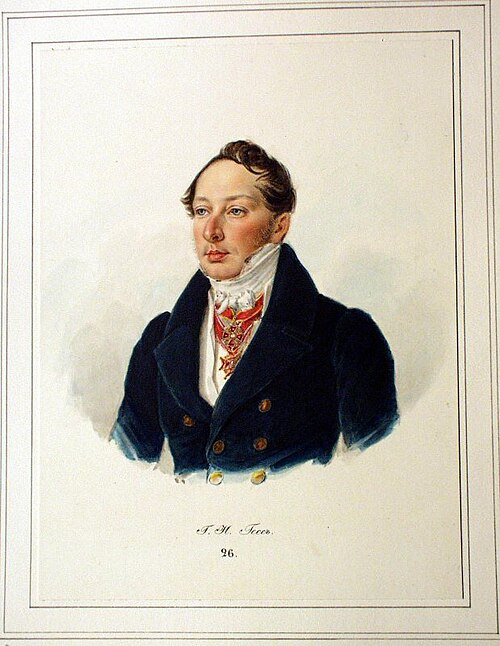
\includegraphics[width=\linewidth]{images/book3/hess.jpg}
\end{minipage}\hfill
\begin{minipage}[t]{0.76\linewidth}\vspace{0pt}
جرمان هنري هس (1802--1850)، أستاذ الكيمياء في سانت بطرسبورغ، قاس
الحرارة المنطلقة عند تخفيف حمض الكبريتيك أو تعديله على عدة مراحل،
ووجد سنة 1840 أن المجموع لا يتعلق بالمراحل المتبعة: إنه «قانون ثبات
مجموع الحرارة»، الذي صيغ قبل المبدأ الأول في الترموديناميك نفسه، المبدأ
الذي يفسّره. (لوحة بريشة إ. إ. رايمرز، 1837--1838؛ CC~BY-SA~4.0،
ويكيميديا كومنز.)
\end{minipage}
\end{history}

\section{حساب أنتالبيات التفاعل}

\subsection*{من أنتالبيات الروابط}

حين ينقص أنتالبي تكوين مركب ما، تعطي طاقة روابطه تقديرًا له، في الطور
الغازي.

\begin{definition}[أنتالبي تفكك الرابطة، متوسط أنتالبي الرابطة]\label{def:b2:reaction-enthalpy:bond-enthalpy}
\emph{أنتالبي تفكك الرابطة}\index{أنتالبي تفكك الرابطة} A--B في جزيء غازي
هو \omterm{def:b2:reaction-enthalpy:standard-reaction-enthalpy}{أنتالبي التفاعل القياسي} لكسر هذه الرابطة إلى جزأين غازيين،
\ce{AB(g) -> A(g) + B(g)} في جزيء ثنائي الذرة. وحين يحوي جزيء $n$ روابط
متماثلة، يكون \emph{متوسط أنتالبي الرابطة}\index{متوسط أنتالبي الرابطة}
فيه هو الأنتالبي القياسي لتذريته الكاملة إلى ذرات غازية مقسومًا على
$n$.
\end{definition}

أنتالبيات التذرية هي نفسها أنتالبيات تكوين: أنتالبيات تكوين الذرات
الغازية، ناقص أنتالبي تكوين الجزيء. والجدول أدناه محسوب بهذه الطريقة.

\begin{omfigure}
\begin{tabular}{lrl}
\hline
الرابطة & الأنتالبي (\unit{kJ/mol}) & مصدر القيمة \\
\hline
H--H & 436 & \ce{H2}، تفكك \\
O=O & 498 & \ce{O2}، تفكك \\
N$\equiv$N & 945 & \ce{N2}، تفكك \\
Cl--Cl & 243 & \ce{Cl2}، تفكك \\
H--Cl & 432 & \ce{HCl}، تفكك \\
C--H & 416 & \ce{CH4}، متوسط أربع روابط \\
N--H & 391 & \ce{NH3}، متوسط ثلاث روابط \\
O--H & 464 & \ce{H2O}، متوسط رابطتين \\
C=O & 804 & \ce{CO2}، متوسط رابطتين \\
C--C & 330 & \ce{C2H6}، مع أخذ C--H من الميثان \\
C=C & 589 & \ce{C2H4}، مع أخذ C--H من الميثان \\
\hline
\end{tabular}

\smallskip
{\small أنتالبيات الروابط عند \qty{298.15}{K}، محسوبة من أنتالبيات التكوين
القياسية للذرات والجزيئات الغازية. ويُظهر السطران الأخيران حدّ
الطريقة: فرابطة C--H في الإيثان ليست تمامًا رابطة C--H في الميثان،
وقيمة C--C ترث الفرق.}
% ledger: dfh:C_g, janaf:H, dfh:O_g, dfh:N_g, janaf:Cl, janaf:HCl, dfh:CH4_g, dfh:NH3_g, dfh:H2O_g, dfh:CO2, dfh:C2H6_g, dfh:C2H4_g (computed in figdata/bachelor-2/thermo-data.py)
\end{omfigure}

\begin{proposition}[التقدير من أنتالبيات الروابط]\label{prop:b2:reaction-enthalpy:bond-estimate}
من أجل تفاعل بين غازات،
\[
  \Delta_r H^\circ \approx \sum(\text{أنتالبيات الروابط المكسورة}) -
  \sum(\text{أنتالبيات الروابط المتكوّنة}).
\]
\end{proposition}

\begin{proof}
لنتبع المسار الذي يذرّي كل متفاعل (الأنتالبي: الروابط المكسورة) ثم يبني
النواتج من الذرات (ناقص الروابط المتكوّنة). يجعل \omterm{thm:b2:reaction-enthalpy:hess}{قانون هس} المجموع مضبوطًا
حين يكون أنتالبي كل رابطة هو أنتالبي الرابطة في جزيئها نفسه؛ واستبداله
بقيمة متوسطة مأخوذة من جزيء آخر هو التقريب.
\end{proof}

\begin{example}[هدرجة الإيثين]\label{ex:b2:reaction-enthalpy:hydrogenation}
في \ce{C2H4(g) + H2(g) -> C2H6(g)}، تُكسر رابطة C=C واحدة ورابطة H--H
واحدة وتحل محلهما رابطة C--C واحدة ورابطتا C--H. وبالجدول: $589 + 436 - 330 - 2
\times 416 = \qty{-137}{kJ/mol}$؛ ومن أنتالبيات التكوين تكون القيمة
\qty{-136.3}{kJ/mol}. والاتفاق جيد هنا لأن قيمتي C--C وC=C في الجدول
أُخذتا من هذين الجزيئين بالذات؛ أما في جزيء لا يشبه جزيئات الجدول فخطأ
من 10 إلى \qty{30}{kJ/mol} أمر شائع.
% ledger: dfh:C2H4_g, dfh:C2H6_g
\end{example}

\subsection*{أنتالبيات الشبكة: دورة بورن--هابر}

\begin{definition}[أنتالبي الشبكة]\label{def:b2:reaction-enthalpy:lattice-enthalpy}
\emph{أنتالبي الشبكة}\index{أنتالبي الشبكة} لبلورة أيونية هو \omterm{def:b2:reaction-enthalpy:standard-reaction-enthalpy}{أنتالبي التفاعل
القياسي} لتفككها إلى أيونات غازية: ففي كلوريد الصوديوم،
\ce{NaCl(s) -> Na+(g) + Cl-(g)}. وهو موجب، ويقيس تماسك البلورة.
\end{definition}

لا يمكن قياسه مباشرة، لكن دورة عبر العناصر تعطيه انطلاقًا من مقادير
قابلة للقياس: أنتالبي تكوين البلورة، وتذرية العناصر، وطاقة تأين الفلز،
والألفة الإلكترونية للافلز (وكلتاهما معرّفتان في مجلد السنة الأولى).

\begin{omfigure}
\begin{tikzpicture}[font=\small, >={Stealth}, y=0.0058cm]
  \def\lw{5.0}
  % levels (kJ/mol relative to Na(s) + 1/2 Cl2(g))
  \draw[thick] (0,0) -- (\lw,0) node[right] {\ce{Na(s) + 1/2Cl2(g)}};
  \draw[thick] (0,107.5) -- (\lw,107.5) node[right] {\ce{Na(g) + 1/2Cl2(g)}};
  \draw[thick] (0,228.8) -- (\lw,228.8) node[right] {\ce{Na(g) + Cl(g)}};
  \draw[thick] (0,724.6) -- (\lw,724.6) node[right] {\ce{Na+(g) + e- + Cl(g)}};
  \draw[thick] (0,376.1) -- (\lw,376.1) node[right] {\ce{Na+(g) + Cl-(g)}};
  \draw[thick] (0,-411.1) -- (\lw,-411.1) node[right] {\ce{NaCl(s)}};
  % the path through the elements, on the left
  \draw[->, omDef] (0.4,0) -- (0.4,107.5);
  \node[omDef, left, font=\footnotesize] at (0.35,53) {\foreignlanguage{arabic}{تسامٍ $107.5$}};
  \draw[->, omDef] (0.4,107.5) -- (0.4,228.8);
  \node[omDef, left, font=\footnotesize] at (0.35,168) {\foreignlanguage{arabic}{$\tfrac12$ تفكك $121.3$}};
  \draw[->, omDef] (0.4,228.8) -- (0.4,724.6);
  \node[omDef, left, font=\footnotesize] at (0.35,480) {\foreignlanguage{arabic}{تأين \babelsublr{Na} $495.8$}};
  \draw[->, omThm] (1.4,724.6) -- (1.4,376.1);
  \node[omThm, right, font=\footnotesize] at (1.45,560) {\foreignlanguage{arabic}{اكتساب إلكترون $-348.6$}};
  \draw[->, omProp] (2.3,0) -- (2.3,-411.1);
  \node[omProp, left, font=\footnotesize] at (2.25,-205) {\foreignlanguage{arabic}{تكوين $-411.1$}};
  % the lattice enthalpy, the only unknown
  \draw[->, thick] (3.6,-411.1) -- (3.6,376.1);
  \node[right, font=\footnotesize] at (3.65,-205) {\foreignlanguage{arabic}{أنتالبي الشبكة $787$}};
\end{tikzpicture}

{\small دورة بورن--هابر لكلوريد الصوديوم عند \qty{298}{K}
(\unit{kJ/mol}). الصعود من البلورة إلى الأيونات الغازية \omterm{def:b2:reaction-enthalpy:lattice-enthalpy}{بأنتالبي الشبكة}،
أو الالتفاف عبر العناصر، يقود إلى المستوى نفسه: \omterm{def:b2:reaction-enthalpy:lattice-enthalpy}{فأنتالبي الشبكة} هو
المجهول الوحيد في الدورة.}
% ledger: dfh:NaCl_cr, dfh:Na_g, janaf:Cl, ie:Na, ea:Cl
\end{omfigure}

\begin{method}[دورة بورن--هابر]\label{met:b2:reaction-enthalpy:born-haber}
\begin{enumerate}
  \item انطلاقًا من العناصر في حالاتها المرجعية، ارسم مسارين: أحدهما
        إلى البلورة (التكوين)، والآخر إلى الأيونات الغازية (تسامي الفلز،
        وتذرية اللافلز، والتأين، واكتساب الإلكترون).
  \item أغلق الدورة \omterm{def:b2:reaction-enthalpy:lattice-enthalpy}{بأنتالبي الشبكة}، من البلورة صعودًا إلى الأيونات
        الغازية.
  \item اكتب أن مجموع الأنتالبيات على طول الدورة معدوم، واستخرج
        المجهول. طاقات التأين والألفات الإلكترونية مجدولة بوحدة eV لكل
        ذرة: اضربها في $N_A e = \qty{96.485}{kJ/(mol.eV)}$.
\end{enumerate}
\end{method}

\begin{example}[كلوريد الصوديوم]\label{ex:b2:reaction-enthalpy:nacl}
$\Delta_{\text{شبكة}}H^\circ = 411.1 + 107.5 + 121.3 + 495.8 - 348.6 =
\qty{787}{kJ/mol}$. وطاقة التأين والألفة الإلكترونية طاقتان عند
\qty{0}{K}؛ وتصحيحاهما إلى \qty{298}{K} ($+\tfrac52RT$ لكل منهما)
يُختصران بين المرحلتين. ويعطي نموذج بلوري بشحنات نقطية قيمة قريبة، ولهذا
يُسمّى كلوريد الصوديوم أيونيًا.
% ledger: dfh:NaCl_cr, dfh:Na_g, janaf:Cl, ie:Na, ea:Cl (computed in figdata/bachelor-2/thermo-data.py)
\end{example}

\section{أنتالبيات التفاعل ودرجة الحرارة}

تعطي الجداول $\Delta_f H^\circ$ عند \qty{298.15}{K}. ويعمل مفاعل عند
\qty{700}{K}، ولهب عند \qty{2000}{K}: فكيف يتغير $\Delta_r H^\circ$ مع
درجة الحرارة؟

\begin{theorem}[قانون كيرشوف]\label{thm:b2:reaction-enthalpy:kirchhoff}
لدينا
\[
  \frac{\dd\Delta_r H^\circ}{\dd T} = \Delta_r C_p^\circ =
  \sum_i\nu_i C_{p,m,i}^\circ ,
\]
بحيث $\Delta_r H^\circ(T_2) = \Delta_r H^\circ(T_1) + \int_{T_1}^{T_2}
\Delta_r C_p^\circ\,\dd T$ (\emph{قانون كيرشوف}\index{قانون كيرشوف})،
في غياب أي تغيّر للحالة الفيزيائية بين $T_1$ و$T_2$.
\end{theorem}

\begin{proof}
وكل نوع كيميائي في حالته القياسية، تكون $H^\circ(T, \xi) = \sum_in_i
H^\circ_{m,i}(T)$ دالة لمتغيرين مشتقاتها الجزئية الثانية متصلة؛ وحسب
مبرهنة شفارتز تتبادل هذه المشتقات:
\[
  \frac{\dd\Delta_r H^\circ}{\dd T} = \frac{\partial}{\partial T}
  \frac{\partial H^\circ}{\partial\xi} = \frac{\partial}{\partial\xi}
  \frac{\partial H^\circ}{\partial T} = \frac{\partial}{\partial\xi}
  \sum_in_iC^\circ_{p,m,i} = \sum_i\nu_iC^\circ_{p,m,i}.
\]
وبالمكاملة بين $T_1$ و$T_2$ نحصل على الصيغة الثانية. وتغيّر الحالة
الفيزيائية لنوع كيميائي داخل الفترة يضيف أنتالبي تحوّله، مضروبًا في
عدده الستوكيومتري.
\end{proof}

\begin{example}[تخليق الأمونيا على الساخن]\label{ex:b2:reaction-enthalpy:kirchhoff}
من أجل \ce{N2(g) + 3H2(g) -> 2NH3(g)}، $\Delta_r H^\circ(298) =
\qty{-91.9}{kJ/mol}$، ومع السعات الحرارية عند \qty{298}{K}،
$\Delta_r C_p^\circ = 2(35.65) - 29.12 - 3(28.84) =
\qty{-44.3}{J/(K.mol)}$. وبعدّه ثابتًا نحصل على $\Delta_r
H^\circ(700) = -91.9 - 0.0443 \times 402 = \qty{-109.7}{kJ/mol}$. أما
الجداول، التي تتابع السعات الحرارية في ازديادها مع درجة الحرارة، فتعطي
\qty{-105.2}{kJ/mol}: فالتقدير بسعة $C_p$ ثابتة يخطئ بنسبة 4\,\%، وهو ثمن
معقول لحساب من سطر واحد. وعلى مدى \qty{400}{K}، يتغير \omterm{def:b2:reaction-enthalpy:reaction-quantity}{أنتالبي التفاعل}
بنحو السُّبع.
% ledger: dfh:NH3_g, cp:NH3_g.298, cp:N2_g.298, cp:H2_g.298, janafdfH:NH3.700 (computed in figdata/bachelor-2/thermo-data.py)
\end{example}

\section{التفاعلات الكظومة والمسعرية}

\subsection*{درجة حرارة اللهب}

في اللهب يكون التفاعل سريعًا ولا يتسع الوقت للحرارة كي تغادر: فالغازات
تسخّن نفسها.

\begin{definition}[درجة حرارة اللهب الكظومة]\label{def:b2:reaction-enthalpy:flame-temperature}
\emph{درجة حرارة اللهب الكظومة}\index{درجة حرارة اللهب الكظومة} لوقود هي
درجة الحرارة التي تبلغها نواتج احتراقه التام حين يجري التفاعل عند ضغط
ثابت، دون أي تبادل للحرارة، انطلاقًا من متفاعلات عند \qty{298}{K}.
\end{definition}

\begin{proposition}[حساب درجة حرارة لهب]\label{prop:b2:reaction-enthalpy:flame}
إذا تقدم التفاعل بمقدار $\xi$ انطلاقًا من متفاعلات عند $T_0$ وكانت
السعة الحرارية للنظام النهائي $C_p(T)$، فإن درجة الحرارة النهائية $T_f$
تحقق
\[
  \xi\,\Delta_r H^\circ(T_0) + \int_{T_0}^{T_f}C_p(T)\,\dd T = 0 .
\]
\end{proposition}

\begin{proof}
التحوّل كظوم وعند ضغط ثابت، فيكون $\Delta H =
Q_p = 0$. ولأن $H$ دالة حالة، فإن أي مسار بين الحالتين الابتدائية
والنهائية نفسيهما يعطي $\Delta H$ نفسه. لنأخذ مسار الشكل أدناه: أولًا
التفاعل عند $T_0$، مع
$\Delta H_1 = \xi\Delta_r H^\circ(T_0)$ (\cref{prop:b2:reaction-enthalpy:qp}،
مع سلوك مثالي)؛ ثم تسخين النظام النهائي من $T_0$ إلى
$T_f$، $\Delta H_2 = \int C_p\,\dd T$. ومجموعهما معدوم.
\end{proof}

\begin{omfigure}
\begin{tikzpicture}[font=\small, >={Stealth}]
  \draw[->] (0,0) -- (6.2,0) node[right] {\foreignlanguage{arabic}{التقدم $\xi$}};
  \draw[->] (0,0) -- (0,3.6) node[above] {\foreignlanguage{arabic}{درجة الحرارة $T$}};
  \fill (0.6,0.6) circle (2pt) node[below left] {\foreignlanguage{arabic}{المتفاعلات، $T_0$}};
  \fill (5.2,0.6) circle (2pt) node[below] {\foreignlanguage{arabic}{النواتج، $T_0$}};
  \fill (5.2,3.0) circle (2pt) node[right] {\foreignlanguage{arabic}{النواتج، $T_f$}};
  \draw[->, thick, omDef] (0.7,0.6) -- (5.1,0.6);
  \node[omDef, above, font=\footnotesize] at (3.15,0.64) {$\Delta H_1 = \xi\,\Delta_r H^\circ(T_0) < 0$};
  \draw[->, thick, omThm] (5.2,0.7) -- (5.2,2.9);
  \node[omThm, right, align=left] at (5.25,1.8) {$\Delta H_2 = \int_{T_0}^{T_f} C_p\,\dd T$};
  \draw[->, thick, dashed] (0.75,0.75) -- (5.05,2.92);
  \node[above left, align=center] at (2.6,1.75) {\foreignlanguage{arabic}{لهب حقيقي:}\\ $\Delta H = 0$};
\end{tikzpicture}

{\small اللهب الكظوم (المتقطع) ومسار مكافئ عبر مرحلتين: التفاعل عند درجة
حرارة ثابتة، ثم تسخين النواتج. ولأن $H$ دالة حالة، فإن مجموع تغيّري
الأنتالبي في المرحلتين معدوم.}
\end{omfigure}

\begin{method}[درجة حرارة اللهب]\label{met:b2:reaction-enthalpy:flame-temperature}
\begin{enumerate}
  \item اكتب الاحتراق التام لمول واحد من الوقود؛ وفي الهواء أضف
        النيتروجين والأرغون اللذين يرافقان الأكسجين (فهما يُسخَّنان
        أيضًا)؛ وخذ الماء بخارًا.
  \item احسب $q = -\Delta_r H^\circ(T_0)$ لكل مول من الوقود.
  \item إما أن تأخذ سعة حرارية ثابتة $C_p$ للنواتج:
        $T_f = T_0 + q/C_p$؛ وإما أن تجد بالاستيفاء $T_f$ التي يساوي عندها
        مجموعُ الزيادات المجدولة $n_i[H^\circ_{m,i}(T_f) - H^\circ_{m,i}(T_0)]$
        المقدارَ $q$.
\end{enumerate}
\end{method}

\begin{omfigure}
\begin{tikzpicture}
\begin{axis}[
  width=0.8\linewidth, height=6.2cm, xmin=300, xmax=3000, ymin=0, ymax=3200,
  axis x line=bottom, axis y line=left, xlabel={\babelsublr{$T$ (K)}},
  ylabel={\foreignlanguage{arabic}{$H(T) - H(\qty{298}{K})$ للنواتج \babelsublr{(kJ)}}},
  xtick={500,1000,1500,2000,2500,3000},
  tick label style={font=\small}, label style={font=\small}, clip=false,
  legend style={font=\scriptsize, draw=none, at={(0.5,1.03)}, anchor=south}, legend columns=2]
\addplot[omDef, very thick] table[x=T, y=H] {figdata/out/bachelor-2-flame-temperature-butane.dat};
\addplot[omThm, very thick] table[x=T, y=H] {figdata/out/bachelor-2-flame-temperature-methane.dat};
\legend{{مول واحد من البوتان في الهواء}, {مول واحد من الميثان في الهواء}}
\draw[omDef, dashed] (axis cs:300,2657.6) -- (axis cs:3000,2657.6);
\node[omDef, anchor=south east, font=\scriptsize] at (axis cs:2350,2657.6) {$-\Delta_r H^\circ = \qty{2657.6}{kJ}$};
\draw[omDef, dotted] (axis cs:2401,0) -- (axis cs:2401,2657.6);
\fill[omDef] (axis cs:2401,2657.6) circle (1.5pt);
\node[omDef, anchor=north west, font=\scriptsize] at (axis cs:2420,2620) {\qty{2401}{K}};
\draw[omThm, dashed] (axis cs:300,802.3) -- (axis cs:3000,802.3);
\node[omThm, anchor=south west, font=\scriptsize] at (axis cs:320,802.3) {$-\Delta_r H^\circ = \qty{802.3}{kJ}$};
\draw[omThm, dotted] (axis cs:2329,0) -- (axis cs:2329,802.3);
\fill[omThm] (axis cs:2329,802.3) circle (1.5pt);
\node[omThm, anchor=north west, font=\scriptsize] at (axis cs:2350,760) {\qty{2329}{K}};
\end{axis}
\end{tikzpicture}

{\small الأنتالبي اللازم لتسخين نواتج احتراق مول واحد من الوقود (ثنائي
أكسيد الكربون، وبخار الماء، ونيتروجين الهواء وأرغونه) انطلاقًا من
\qty{298}{K}، محسوبًا من الأنتالبيات المجدولة. يلتقي كل منحنى بالحرارة
التي يحررها احتراق وقوده عند \omterm{def:b2:reaction-enthalpy:flame-temperature}{درجة حرارة اللهب الكظومة}: نحو \qty{2400}{K}
للبوتان، و\qty{2330}{K} للميثان.}
% ledger: janafH:CO2.2400, janafH:H2O.2400, janafH:N2.2400, janafH:Ar.2400, air:N2, air:O2, air:Ar (computed in figdata/bachelor-2/flame-temperature.py)
\end{omfigure}

درجات الحرارة المحسوبة حدود عليا. ففوق نحو \qty{2000}{K} يبدأ ثنائي
أكسيد الكربون والماء بالتفكك إلى أحادي أكسيد الكربون والهيدروجين
والأكسجين وجذور حرة؛ وهذه التفاعلات الماصة للحرارة تسترجع جزءًا من
الحرارة، فيكون لهب البوتان الحقيقي في الهواء أبرد بوضوح مما يُحسب. وفي
الأكسجين النقي لا يوجد نيتروجين يُسخَّن فيكون اللهب أسخن بكثير، ولهذا
يحرق اللحّامون الإيثاين بالأكسجين لا بالهواء.

\subsection*{المسعرية}

\begin{proposition}[حجم ثابت وضغط ثابت]\label{prop:b2:reaction-enthalpy:bomb}
في وعاء فولاذي مغلق (مسعر القنبلة) تكون الحرارة المقيسة $Q_V =
\Delta U$، ومن أجل الغازات المثالية والأطوار المكثفة
\[
  \Delta_r H = \Delta_r U + \Delta\nu_{\text{غاز}}\,RT ,
\]
حيث $\Delta\nu_{\text{غاز}}$ مجموع الأعداد الستوكيومترية للأنواع
الغازية.
\end{proposition}

\begin{proof}
$H = U + pV$، و$\Delta_r H = \Delta_r U + \partial(pV)/\partial\xi$ عند
$T$ ثابتة. والجداء $pV$ للأطوار المكثفة مهمل، وللغازات
$pV = n_{\text{غاز}}RT$ مع $n_{\text{غاز}} = n_{\text{غاز},0} +
\Delta\nu_{\text{غاز}}\xi$، ومشتقته بالنسبة إلى $\xi$ هي
$\Delta\nu_{\text{غاز}}RT$.
\end{proof}

\begin{omfigure}
\begin{tikzpicture}[font=\small, >={Stealth}, scale=1.0]
  % outer insulated jacket
  \draw[thick, fill=gray!8] (-2.6,-0.2) rectangle (2.6,4.4);
  \draw[thick, fill=white] (-2.3,0.1) rectangle (2.3,4.1);
  % water bath
  \fill[omDef!12] (-2.3,0.1) rectangle (2.3,3.4);
  \draw[omDef!60] (-2.3,3.4) -- (2.3,3.4);
  % bomb
  \draw[very thick, fill=gray!35] (-0.75,0.5) rectangle (0.75,2.6);
  \draw[very thick, fill=gray!55] (-0.9,2.6) rectangle (0.9,2.85);
  \draw[thick] (-0.3,1.0) -- (-0.3,1.9) (0.3,1.0) -- (0.3,1.9);
  \draw[thick, fill=orange!50] (-0.3,0.95) rectangle (0.3,1.05);
  \draw[red!70!black, thick, decorate, decoration={zigzag, amplitude=1pt, segment length=3pt}] (-0.3,1.9) -- (0.3,1.9);
  % wires
  \draw (-0.3,2.85) -- (-0.3,4.7) (0.3,2.85) -- (0.3,4.7);
  % stirrer and thermometer
  \draw[thick] (1.6,0.6) -- (1.6,4.7);
  \draw[thick, fill=gray!40] (1.35,0.55) rectangle (1.85,0.75);
  \pic[transform shape] at (-1.6,0.4) {thermometer};
  % labels
  \draw (-0.75,1.6) -- (-3.3,1.6) node[left] {\foreignlanguage{arabic}{قنبلة فولاذية، \ce{O2} تحت \babelsublr{30 bar}}};
  \draw (0,1.0) -- (-3.3,0.6) node[left] {العيّنة في بوتقتها};
  \draw (0,1.9) -- (-3.3,2.6) node[left] {سلك الإشعال};
  \draw (1.0,3.0) -- (3.3,3.0) node[right] {حمام مائي};
  \draw (1.6,3.9) -- (3.3,4.3) node[right] {المحرِّك};
  \draw (-1.6,3.4) -- (-3.3,3.6) node[left] {محرار};
  \draw (2.45,0.3) -- (3.3,0.5) node[right] {غلاف عازل};
\end{tikzpicture}

{\small مسعر القنبلة. تحترق العيّنة عند حجم ثابت في أكسجين تحت الضغط؛
وتذهب الحرارة إلى القنبلة وإلى الماء المحرَّك، الذي يُقرأ ارتفاع درجة
حرارته على المحرار. وتُعيَّن السعة الحرارية للمسعر مسبقًا بحرق مادة
معيارية معلومة الطاقة.}
\end{omfigure}

\begin{method}[المسعرية]\label{met:b2:reaction-enthalpy:calorimetry}
\begin{enumerate}
  \item عايِر: احرق كتلة من مادة معيارية معلومة طاقة الاحتراق (أو مرّر
        طاقة كهربائية معلومة)، واقرأ ارتفاع درجة الحرارة $\Delta T$،
        واستنتج السعة الحرارية $C$ للمسعر كله (الماء والوعاء، أي
        «المكافئ المائي» للمسعر).
  \item احرق العيّنة، واقرأ $\Delta T'$: الحرارة المحررة هي $C\,\Delta
        T'$، ومنه $\Delta_r U = -C\Delta T'/\xi$ عند حجم ثابت.
  \item صحّح إلى $\Delta_r H$ بالحد $\Delta\nu_{\text{غاز}}RT$؛ وفي مسعر
        مفتوح (عند ضغط ثابت) يكون $\Delta_r H = -C\Delta T'/\xi$
        مباشرة.
\end{enumerate}
\end{method}

\begin{example}[قياس بالقنبلة]\label{ex:b2:reaction-enthalpy:bomb}
في احتراق البوتان مع ماء سائل، $\Delta\nu_{\text{غاز}} = 4
- 1 - 6.5 = -3.5$، ومنه $\Delta_r U = \Delta_r H + 3.5RT = -2877.6 + 8.7 =
\qty{-2868.9}{kJ/mol}$: والتصحيح بضعة أجزاء من الألف، وهو أكبر من عدم
يقين قياس جيد بالقنبلة، فلا يُهمل أبدًا.
% ledger: dfh:C4H10_g, dfh:CO2, dfh:H2O-l (computed in figdata/bachelor-2/thermo-data.py)
\end{example}

\begin{history}[القنابل المسعرية، 1881]
\begin{minipage}[t]{0.2\linewidth}\vspace{0pt}
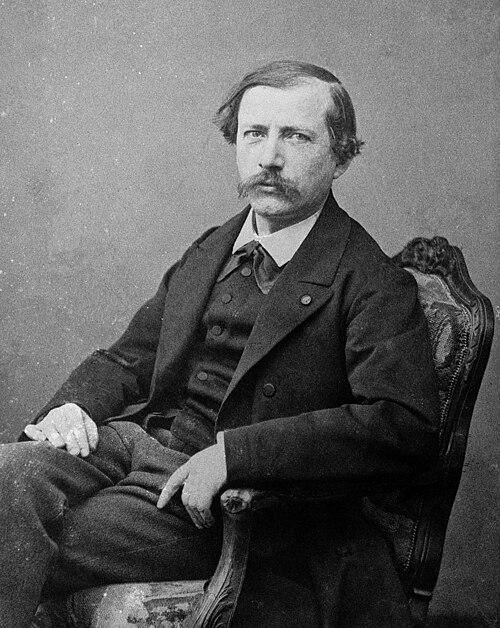
\includegraphics[width=\linewidth]{images/book3/berthelot.jpg}
\end{minipage}\hfill
\begin{minipage}[t]{0.76\linewidth}\vspace{0pt}
مارسلان برتلو (1827--1907) أحرق مركبات عضوية في أكسجين مضغوط داخل وعاء
فولاذي مغلق مبطَّن بالبلاتين، كي يكون الاحتراق تامًا ولا يفلت شيء: إنها
القنبلة المسعرية، التي ما زالت أداة القياس المرجعية لحرارات الاحتراق.
وهو الذي وضع أيضًا مصطلحي «\omterm{def:b2:reaction-enthalpy:exothermic}{ناشر للحرارة}» و«\omterm{def:b2:reaction-enthalpy:exothermic}{ماص للحرارة}». (صورة: ملكية
عامة، ويكيميديا كومنز.)
\end{minipage}
\end{history}

\section{تمارين}

\begin{exercise}[$\star$]\label{exo:b2:reaction-enthalpy:1}
مستعملًا أنتالبيات التكوين القياسية الواردة في الفصل، احسب
$\Delta_r H^\circ$ عند \qty{298}{K} لاحتراق البروبان،
\ce{C3H8(g) + 5O2(g) -> 3CO2(g) + 4H2O(l)}، علمًا أن $\Delta_f
H^\circ(\ce{C3H8}, \text{g}) = \qty{-104.7}{kJ/mol}$. هل التفاعل \omterm{def:b2:reaction-enthalpy:exothermic}{ناشر
للحرارة}؟
% ledger: dfh:C3H8_g
\end{exercise}

\begin{exercise}[$\star$]\label{exo:b2:reaction-enthalpy:2}
احسب الحرارة المحررة بحرق \qty{1.00}{kg} من الميثان (والماء المتكوّن
سائل) و\qty{1.00}{kg} من ثنائي الهيدروجين، \ce{H2(g) + 1/2O2(g) ->
H2O(l)}. أي الوقودين يعطي حرارة أكبر لكل كيلوغرام؟
\end{exercise}

\begin{exercise}[$\star$]\label{exo:b2:reaction-enthalpy:3}
يعطي مسعر قنبلة $\Delta_r U = \qty{-3264}{kJ/mol}$ لاحتراق البنزين
السائل وفق \ce{C6H6(l) + 15/2O2(g) -> 6CO2(g) + 3H2O(l)} عند
\qty{298}{K}. احسب $\Delta_r H$.
\end{exercise}

\begin{exercise}[$\star$]\label{exo:b2:reaction-enthalpy:4}
علمًا أن $\Delta_r H^\circ = \qty{-393.5}{kJ/mol}$ للتفاعل \ce{C(s) + O2(g) ->
CO2(g)} و$\Delta_r H^\circ = \qty{-283.0}{kJ/mol}$ للتفاعل \ce{CO(g) +
1/2O2(g) -> CO2(g)}، احسب \omterm{def:b2:reaction-enthalpy:reaction-quantity}{أنتالبي التفاعل} \ce{CO2(g) + C(s) -> 2CO(g)}،
وهو التفاعل الذي يجري في فحم الكوك الساخن داخل الفرن العالي.
\end{exercise}

\begin{exercise}[$\star\star$]\label{exo:b2:reaction-enthalpy:5}
قدّر بواسطة أنتالبيات الروابط الواردة في الفصل \omterm{def:b2:reaction-enthalpy:reaction-quantity}{أنتالبي التفاعل}
\ce{CH4(g) + Cl2(g) -> CH3Cl(g) + HCl(g)}، آخذًا \qty{350}{kJ/mol} للرابطة
C--Cl. ثم احسب المقدار نفسه من أنتالبيات التكوين، علمًا أن
$\Delta_f H^\circ(\ce{CH3Cl}, \text{g}) = \qty{-83.7}{kJ/mol}$، وعلّق على
الفرق.
% ledger: dfh:CH3Cl_g
\end{exercise}

\begin{exercise}[$\star\star$]\label{exo:b2:reaction-enthalpy:6}
أنتالبي التبخير القياسي للماء عند \qty{298}{K} هو
$\Delta_f H^\circ(\ce{H2O}, \text{g}) - \Delta_f H^\circ(\ce{H2O},
\text{l})$. احسبه. ثم قدّره عند \qty{400}{K} (ماء فائق التسخين تحت الضغط)
مع $C_{p,m}^\circ = \qty{75.35}{J/(K.mol)}$ للسائل
و\qty{33.59}{J/(K.mol)} للبخار، وكلتاهما ثابتة، وقارن بالجداول، التي
تعطي $\Delta_f H^\circ =
\qty{-282.59}{kJ/mol}$ للسائل و\qty{-242.85}{kJ/mol} للبخار عند
\qty{400}{K}.
% ledger: cp:H2O_l.298, cp:H2O_g.298, janafdfH:H2O_l.400, janafdfH:H2O_g.400
\end{exercise}

\begin{exercise}[$\star\star$]\label{exo:b2:reaction-enthalpy:7}
استعمل دورة بورن--هابر لحساب \omterm{def:b2:reaction-enthalpy:lattice-enthalpy}{أنتالبي الشبكة} لكلوريد البوتاسيوم انطلاقًا
من: $\Delta_f H^\circ(\ce{KCl}, \text{s}) = \qty{-436.7}{kJ/mol}$، وتسامي
البوتاسيوم \qty{89.0}{kJ/mol}، وطاقة تأين البوتاسيوم \qty{4.341}{eV}،
و$\Delta_f H^\circ(\ce{Cl}, \text{g}) =
\qty{121.3}{kJ/mol}$، والألفة الإلكترونية للكلور \qty{3.613}{eV}. لماذا هو
أصغر من أنتالبي شبكة كلوريد الصوديوم؟
% ledger: dfh:KCl_cr, dfh:K_g, ie:K, janaf:Cl, ea:Cl
\end{exercise}

\begin{exercise}[$\star\star$]\label{exo:b2:reaction-enthalpy:8}
يُعايَر مسعر من نوع «كوب القهوة» بتمرير \qty{2.00}{kJ} من الطاقة
الكهربائية، فترتفع درجة حرارته بمقدار \qty{0.418}{K}. ثم يُمزج فيه
\qty{50.0}{mL} من حمض الهيدروكلوريك بتركيز \qty{1.00}{mol/L} مع
\qty{50.0}{mL} من محلول هيدروكسيد الصوديوم بتركيز \qty{1.10}{mol/L}،
وكلاهما عند درجة الحرارة الابتدائية نفسها: فترتفع درجة الحرارة بمقدار
\qty{0.583}{K}. احسب \omterm{def:b2:reaction-enthalpy:reaction-quantity}{أنتالبي التفاعل} \ce{H3O+(aq) + OH-(aq) ->
2H2O(l)}.
\end{exercise}

\begin{exercise}[$\star\star$]\label{exo:b2:reaction-enthalpy:9}
للأوكتان، وهو نموذج لوقود السيارات، $\Delta_f H^\circ(\text{l}) =
\qty{-250.3}{kJ/mol}$. احسب أنتالبي احتراقه (والماء سائل)، والحرارة
المحررة لكل كيلوغرام، وكتلة ثنائي أكسيد الكربون المنبعثة لكل ميغاجول.
وقارن بالميثان.
% ledger: dfh:C8H18
\end{exercise}

\begin{exercise}[$\star\star\star$]\label{exo:b2:reaction-enthalpy:10}
احسب \omterm{def:b2:reaction-enthalpy:flame-temperature}{درجة حرارة اللهب الكظومة} للميثان المحترق في الكمية الستوكيومترية
من الأكسجين النقي، بسعات حرارية ثابتة (سعات الفصل عند \qty{298}{K}:
\ce{CO2} 37.13، \ce{H2O(g)}
\qty{33.59}{J/(K.mol)}). وقارن بالنتيجة في الهواء، \qty{2780}{K} بالتقريب
نفسه. لماذا يكون اللهب الحقيقي في الأكسجين أبرد بكثير مما يقوله هذا
الحساب؟
% ledger: cp:CO2_g.298, cp:H2O_g.298
\end{exercise}

\begin{exercise}[$\star\star\star$]\label{exo:b2:reaction-enthalpy:11}
كثيرًا ما تُكتب السعة الحرارية لغاز على الصورة $C_{p,m}^\circ = a + bT$. ومن
أجل تخليق الأمونيا، خذ $\Delta_r a = \qty{-60.5}{J/(K.mol)}$
و$\Delta_r b = \qty{0.0540}{J/(K^2.mol)}$ (مضبوطتين على الجداول بين
\qty{300}{K} و\qty{800}{K}). كامِل \omterm{thm:b2:reaction-enthalpy:kirchhoff}{قانون كيرشوف} من \qty{298}{K} إلى
\qty{700}{K} وقارن بالقيمة الواردة في الجداول، \qty{-105.2}{kJ/mol}،
وبالتقدير بسعة $C_p$ ثابتة.
\end{exercise}

\begin{exercise}[$\star\star\star$]\label{exo:b2:reaction-enthalpy:12}
يتكوّن أحادي أكسيد النيتروجين في المحركات وفق \ce{N2(g) + O2(g) -> 2NO(g)}.
احسب أنتالبي تفاعله القياسي عند \qty{298}{K}. وبيّن أنه إذا كان
$\Delta_r C_p^\circ$ صغيرًا، فإن التفاعل يمتص الحرارة نفسها تقريبًا عند
\qty{2000}{K}؛ ثم قدّر التغير بين \qty{298}{K} و\qty{2000}{K} مستعملًا
السعات الحرارية الواردة في الجداول عند \qty{298}{K}
(\ce{NO} \qty{29.85}{J/(K.mol)}، \ce{N2} 29.12، \ce{O2}
\qty{29.38}{J/(K.mol)}). وفسّر لماذا قد يكون تفاعل \omterm{def:b2:reaction-enthalpy:exothermic}{ماص للحرارة} مشكلةً
في أسخن اللهب بالذات.
% ledger: dfh:NO_g, cp:NO_g.298, cp:N2_g.298, cp:O2_g.298
\end{exercise}

\section{مسألة: خرطوشة غاز التخييم}

\begin{problem}[{مسألة نهاية الأسبوع --- طاقة البوتان، وقياس في مسعر
قنبلة، والماء المسخَّن في قدر، ودرجة حرارة اللهب}]
\label{pb:b2:reaction-enthalpy:1}
يحرق موقد تخييم البوتان من خرطوشة تحوي \qty{230}{g}. معطيات عند
\qty{298}{K} ($\Delta_f H^\circ$ بوحدة \unit{kJ/mol}): \ce{C4H10(g)}
$-125.6$، \ce{CO2(g)} $-393.51$، \ce{H2O(l)} $-285.83$، \ce{H2O(g)}
$-241.83$. الكتل المولية: \ce{C4H10} \qty{58.12}{g/mol}، \ce{H2O}
\qty{18.02}{g/mol}. السعة الحرارية للماء السائل
\qty{75.35}{J/(K.mol)}. الهواء الجاف: \qty{20.95}{\percent} \ce{O2}،
\qty{78.08}{\percent} \ce{N2}، \qty{0.93}{\percent} \ce{Ar} حجمًا. $R = \qty{8.314}{J/(K.mol)}$.
% ledger: dfh:C4H10_g, dfh:CO2, dfh:H2O-l, dfh:H2O_g, cp:H2O_l.298, air:O2, air:N2, air:Ar

\medskip
\noindent\textbf{الجزء الأول --- الوقود.}
\begin{enumerate}
  \item اكتب معادلة الاحتراق التام للبوتان، والماء المتكوّن سائل، من أجل
        مول واحد من البوتان.
  \item احسب أنتالبي تفاعله القياسي عند \qty{298}{K}.
  \item احسبه مرة أخرى والماء المتكوّن بخار، وفسّر الفرق.
  \item احسب الحرارة المحررة لكل غرام من البوتان في كلتا الحالتين.
  \item أي القيمتين تصف موقد التخييم، الذي يغادر ماؤه اللهب بخارًا؟
  \item ما الحرارة التي يمكن أن تحررها الخرطوشة كلها على الموقد؟
\end{enumerate}

\medskip
\noindent\textbf{الجزء الثاني --- قياس.}
تُحرق عيّنة كتلتها \qty{0.500}{g} من البوتان في مسعر قنبلة سعته الحرارية
\qty{10.00}{kJ/K}؛ ويتكثف الماء المتكوّن.
\begin{enumerate}[resume]
  \item ما المقدار الذي يقيسه مسعر القنبلة، ولماذا؟
  \item احسب $\Delta\nu_{\text{غاز}}$ للتفاعل في السؤال 1.
  \item احسب $\Delta_r U$ المتوقع.
  \item احسب الارتفاع المتوقع في درجة حرارة المسعر.
  \item الارتفاع المقروء \qty{2.461}{K}. استنتج $\Delta_r U$
        و$\Delta_r H$ المقيسين، والفرق النسبي عن قيم الجداول.
\end{enumerate}

\medskip
\noindent\textbf{الجزء الثالث --- القدر.}
\begin{enumerate}[resume]
  \item احسب الحرارة اللازمة لرفع درجة حرارة \qty{1.00}{L} من الماء
        (\qty{1.00}{kg}) من \qty{20}{\celsius} إلى \qty{100}{\celsius}.
  \item يحقق الموقد ذلك مستهلكًا \qty{16.0}{g} من البوتان. احسب كفاءته
        (الحرارة التي يستقبلها الماء مقسومة على الحرارة المحررة).
  \item أين تذهب بقية الحرارة؟
  \item كم لترًا من الماء يمكن أن تُغليه الخرطوشة كلها بهذه الكفاءة؟
\end{enumerate}

\medskip
\noindent\textbf{الجزء الرابع --- اللهب.}
\begin{enumerate}[resume]
  \item يحترق البوتان في الكمية الستوكيومترية من الهواء. احسب كميتي
        ثنائي النيتروجين والأرغون اللتين ترافقان ثنائي الأكسجين الذي
        يحتاجه مول واحد من البوتان.
  \item اذكر كميات النواتج، بما فيها النيتروجين والأرغون.
  \item فسّر، بمسار من مرحلتين، لماذا تُستعمل الحرارة التي يحررها
        التفاعل عند \qty{298}{K} (والماء بخار) كلها في تسخين هذه
        الغازات.
  \item مستعملًا السعات الحرارية عند \qty{298}{K}، \ce{CO2} 37.13،
        \ce{H2O(g)} 33.59، \ce{N2} 29.12، \ce{Ar} \qty{20.79}{J/(K.mol)}،
        احسب السعة الحرارية للنواتج.
  \item استنتج درجة حرارة اللهب بسعات حرارية ثابتة.
  \item تعطي زيادات الأنتالبي الواردة في الجداول، لنواتج مول واحد من
        البوتان، \qty{2515.7}{kJ} بين \qty{298}{K} و\qty{2300}{K}،
        و\qty{2655.7}{kJ} بين \qty{298}{K} و\qty{2400}{K}. أوجد درجة
        حرارة اللهب بالاستيفاء الخطي.
  \item لماذا يكون التقدير الأول مرتفعًا أكثر من اللازم؟
  \item لماذا تكون درجة الحرارة المقيسة للهب البوتان أدنى من ذلك أيضًا؟
  \item اذكر \omterm{def:b2:reaction-enthalpy:flame-temperature}{درجة حرارة اللهب الكظومة} للبوتان في الهواء.
\end{enumerate}
\end{problem}
